\begin{frame}
  \frametitle{Parallel planes}
     Planes
     $\mathcal{P}_1: \quad (\textbf{r} - \textbf{r}_1) \cdot \textbf{n}_1 = 0$
     \hspace{2cm}
     $\mathcal{P}_2: \quad (\textbf{r} - \textbf{r}_2) \cdot \textbf{n}_2 = 0$

  \begin{columns}[t]
    \column[T]{6cm}
    \textcolor[rgb]{0.98,0.00,0.00}{Parallel} planes:  \\
    \uncover<2->{$\mathcal{P}_1 || \mathcal{P}_2$ $\Longleftrightarrow$ $\textbf{n}_1$, $\textbf{n}_2$ collinear $\Longleftrightarrow$
    $$\boxed{\textbf{n}_1 \times \textbf{n}_2 = \textbf{0}}$$}
    \uncover<3->{
    \textcolor[rgb]{0.98,0.00,0.00}{Distance} between parallel planes:
    $$d(\mathcal{P}_1,\mathcal{P}_2) =
    |\textbf{\text{proj}}_{\textbf{n}_1} (\textbf{r}_2-\textbf{r}_1)| = $$
    $$=\boxed{\frac{|(\textbf{r}_2-\textbf{r}_1)\cdot \textbf{n}_1|}{|\textbf{n}_1|}}$$}
    \uncover<4->{\textcolor[rgb]{0.98,0.00,0.00}{Scalar} equations:\\
    $\mathcal{P}_1 : \quad ax+by+cz = d_1$\\
    $\mathcal{P}_2 : \quad ax+by+cz = d_2$
    $$\boxed{d(\mathcal{P}_1,\mathcal{P}_2) = \frac{|d_2-d_1|}{\sqrt{a^2+b^2+c^2}}}$$}
    \column[T]{6.5cm}
    \begin{figure}
        \psfrag{cP1}{$\mathcal{P}_1$}
        \psfrag{cP2}{$\mathcal{P}_2$}
        \psfrag{P1}{$P_1(\textbf{r}_1)$}
        \psfrag{P2}{$P_2(\textbf{r}_2)$}
        \psfrag{n1}{$\textbf{n}_1$}
        \psfrag{n2}{$\textbf{n}_2$}
        \psfrag{r12}{$\textbf{r}_2\!-\!\textbf{r}_1$}
        \psfrag{proj}{$\textbf{\text{proj}}_{\bm{n}_1} (\textbf{r}_1\!-\!\textbf{r}_0)$}
        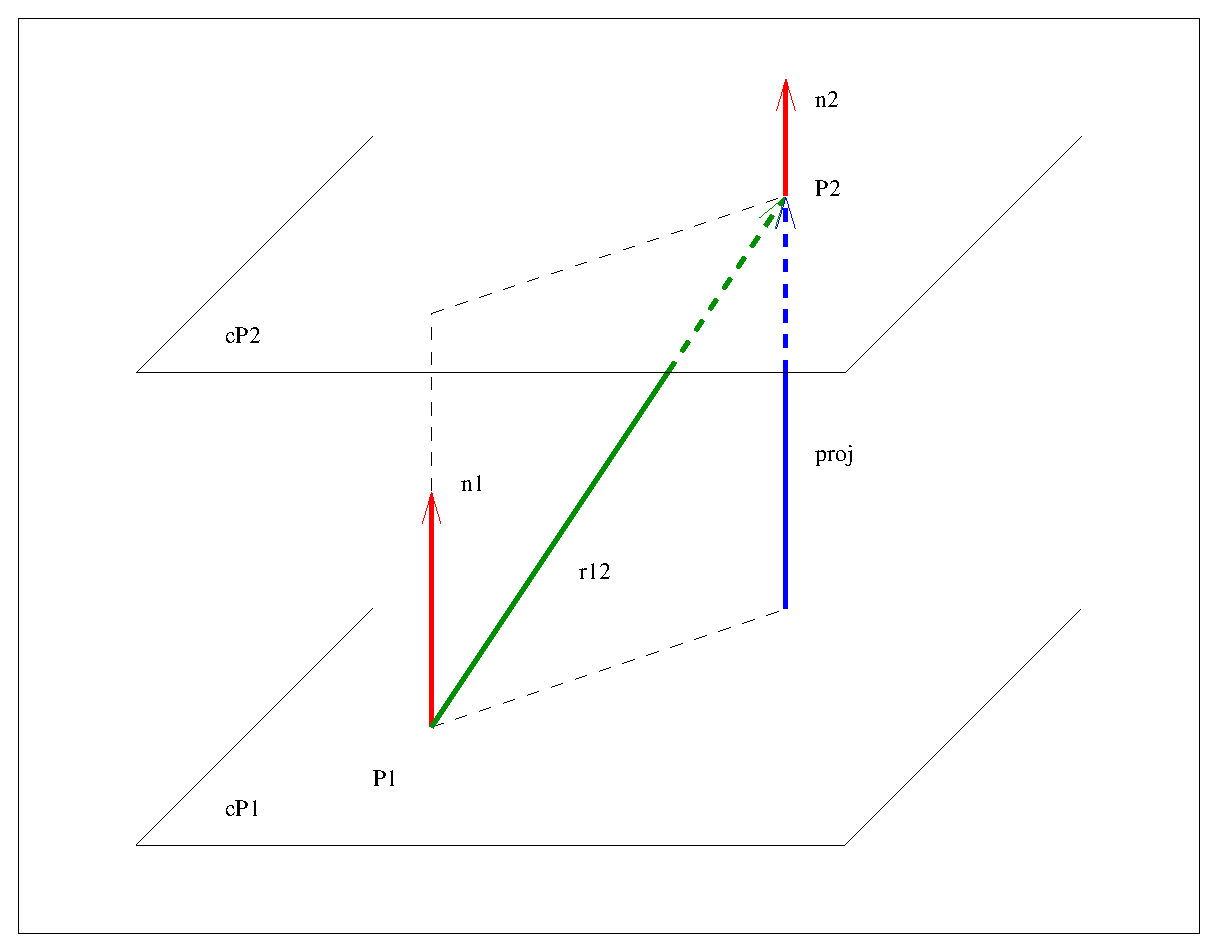
\includegraphics[height=2in]{../../modules/vectors/pictures/ok-parallel_plane_plane.eps}
    \end{figure}
    %
  \end{columns}
\end{frame}